
\chapter{Esto va a ir en otro capítulo que todavía no armé. Y los resultados no estan actualizados}
\section{Comparando resultados entre métodos para barridos de frecuencias}

\section{Verificación del código escrito durante la maestría}

Para ver que todo cierre, obtuve los resultados del paper \cite{Aab_2020} con el código del Rayleigh para distintos bines. En el bin  2 EeV - 4 EeV  tuve incongruencias entre mi código y los valores reportados en el paper, pero si comparo los valores obtenidos con el código utilizado para el paper con mis resultados si se corresponden. En los demás bines los resultados entre el código implementado en \cite{Aab_2020}, los resultados publicados y los resultados de mi código se corresponden.


En el bin 2 EeV - 4 EeV, verifiqué sin cambiaba los números considerando los eventos hasta $80^o$, pero los parámetros de Rayleigh eran los mismos que usar $60^o$  como límite en $\theta$.  Cuando no considero los pesos en mi código, obtengo resultados congruentes con los publicados pero eso puedo ser una casualidad.

\begin{table}[H]
    \begin{small}
        \begin{center}
            \begin{tabular}[c]{l|c|c|c|c|}
                                            & \multicolumn{4}{|c|}{2 EeV - 4 EeV}                                                               \\ \hline
                Frecuencia:                 & Sidérea              & Sidérea (Sin pesos)  & Sidérea \cite{codigo}    & Sidérea \cite{Aab_2020}   \\ \hline
                Amplitud r [\%]:            & $0.5^{+0.3}_{-0.2}$ & $0.4^{+0.3}_{-0.2}$ & $0.5^{+0.3}_{-0.2}$     & -                          \\
                $r_{99}$ [\%]:              & 0.8                 & 0.8                 & 0.8                     & -                          \\\hline
                Amplitud $d_\perp$[\%]:     & $0.7^{+0.4}_{-0.2}$ & $0.5^{+0.4}_{-0.2}$ & $0.7^{+0.4}_{-0.2}$ 	  & $0.5^{+0.4}_{-0.2}$                    \\
                $d_{99}$ [\%]:              & 1.0                 & 1.0                 & 1.0                     & -                         \\
                $d_{\perp,UL}$[\%]:         & 1.9                 & 1.7                 & -                       & 1.4                               \\\hline
                $\sigma_{x,y}$[\%]:         & 0.34	              & 0.34	            & 0.34	                  & 0.34                           \\
                Probabilidad      :         & 0.14                & 0.33                & 0.15               	  & 0.34                       \\
                Fase[$^o$]:                 & 355$\pm$29          & 351$\pm$38          & 346$\pm$29              & 349$\pm$55                    \\\hline
            \end{tabular}
        \end{center}
    \end{small}
    \caption{Características para las frecuencias solar y sidérea con el método Rayleigh en el primer armónico en el rango de energía 2 EeV - 4 EeV, obtenidos con el código de este trabajo \cite{Aab_2020} y comparados con los resultados reportados en el último.}
\end{table}


\begin{table}[H]
    \begin{small}
        \begin{center}
            \begin{tabular}[c]{l|c|c||c|c|}
                                            & \multicolumn{2}{c||}{8 EeV - 16 EeV}              & \multicolumn{2}{c|}{16 EeV - 32 EeV}                   \\ \hline
                Frecuencia:                 & Sidérea                    & Sidérea \cite{Aab_2020} & Sidérea                   & Sidérea \cite{Aab_2020}   \\ \hline
                Amplitud r [\%]:            & $4.4^{+1.0}_{-0.8}$ 	    & -                      & $5.8^{+1.8}_{-1.3}$ 	    & -                         \\
                $r_{99}$ [\%]:              & 2.6                       & -                      & 4.9                      & -                          \\\hline
                Amplitud $d_\perp$[\%]:     & $5.6^{+1.2}_{-1.0}$ 	    & $5.6^{+1.2}_{-1.0}$    & $7.5^{+2.3}_{-1.8}$ 	    & $7.5^{+2.3}_{-1.8}$                   \\
                $d_{99}$ [\%]:              & 3.3                       & -                      & 6.3                      & -                         \\
                $d_{\perp,UL}$[\%]:         & 10                        & -                      & 16                       & -                                 \\\hline
                $\sigma_{x,y}$[\%]:         & 1.1	                    & 1.1                    & 2.1	                    & 2.1                           \\
                Probabilidad      :         & $2.3\times10^{-6}$	    & $2.3\times10^{-6}$     & $1.5\times10^{-3}$	    & $1.5\times10^{-3}$              \\
                Fase[$^o$]:                 & 96$\pm$11                 & 97$\pm$12              & 80$\pm$16                & 80$\pm$17                     \\\hline
            \end{tabular}
        \end{center}
    \end{small}
    \caption{Características para las frecuencias solar y sidérea con el método Rayleigh en el primer armónico en distintos rangos de energía, obtenidos con el código de este trabajo \cite{Aab_2020} y comparados con los resultados reportados en el último.}
\end{table}


\section{Comparando amplitud en función de la frecuencia}

En las Figs.\ref{fig:primer_barrido_EW_Ray}, \ref{fig:segundo_barrido_EW_Ray} y \ref{fig:tercer_barrido_EW_Ray} se comparan el barrido en frecuencia con el método East - West y el barrido con Rayleigh considerando los pesos de los hexágonos en distintos rangos de energía.


\begin{figure}[H]
    \begin{small}
        \begin{center}
            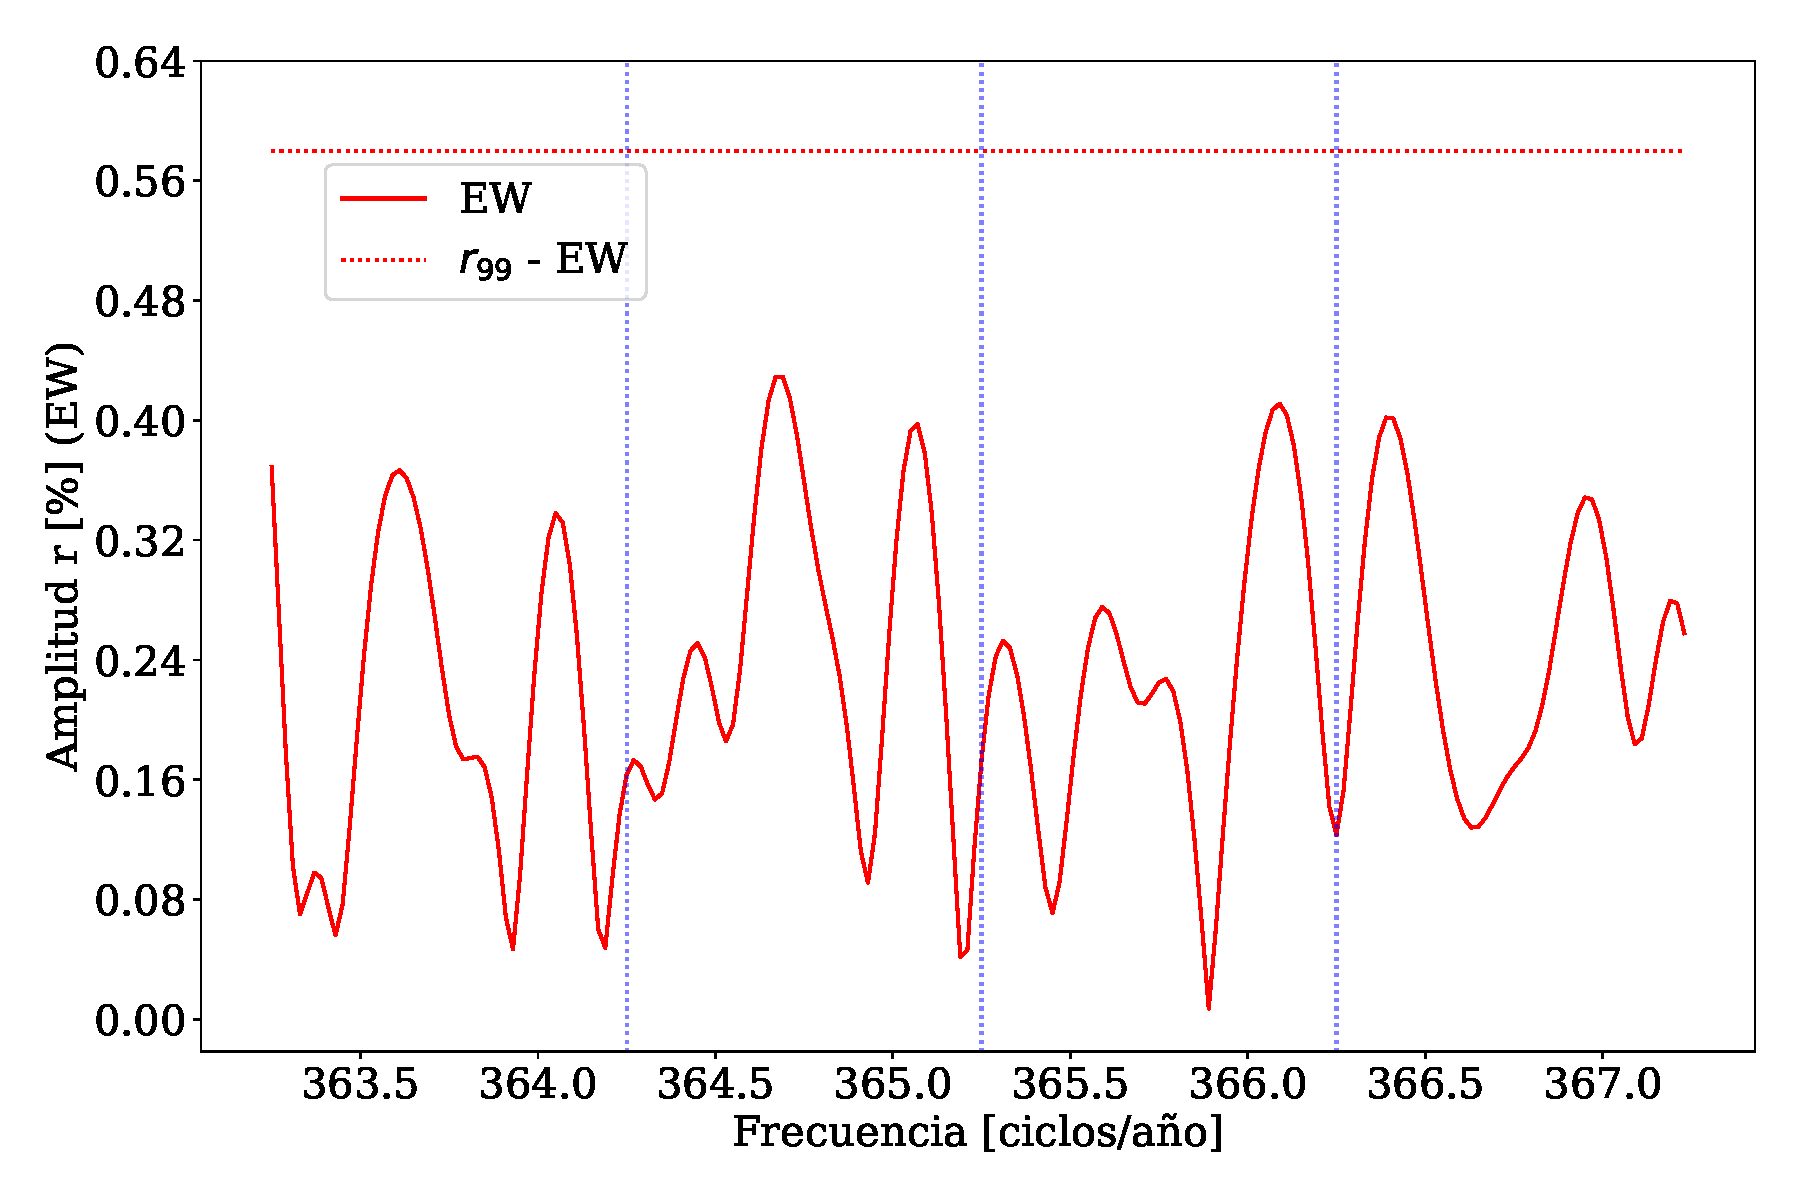
\includegraphics[width=0.4955\textwidth]{plot_bin_1_barrido_v3_EW.pdf}
            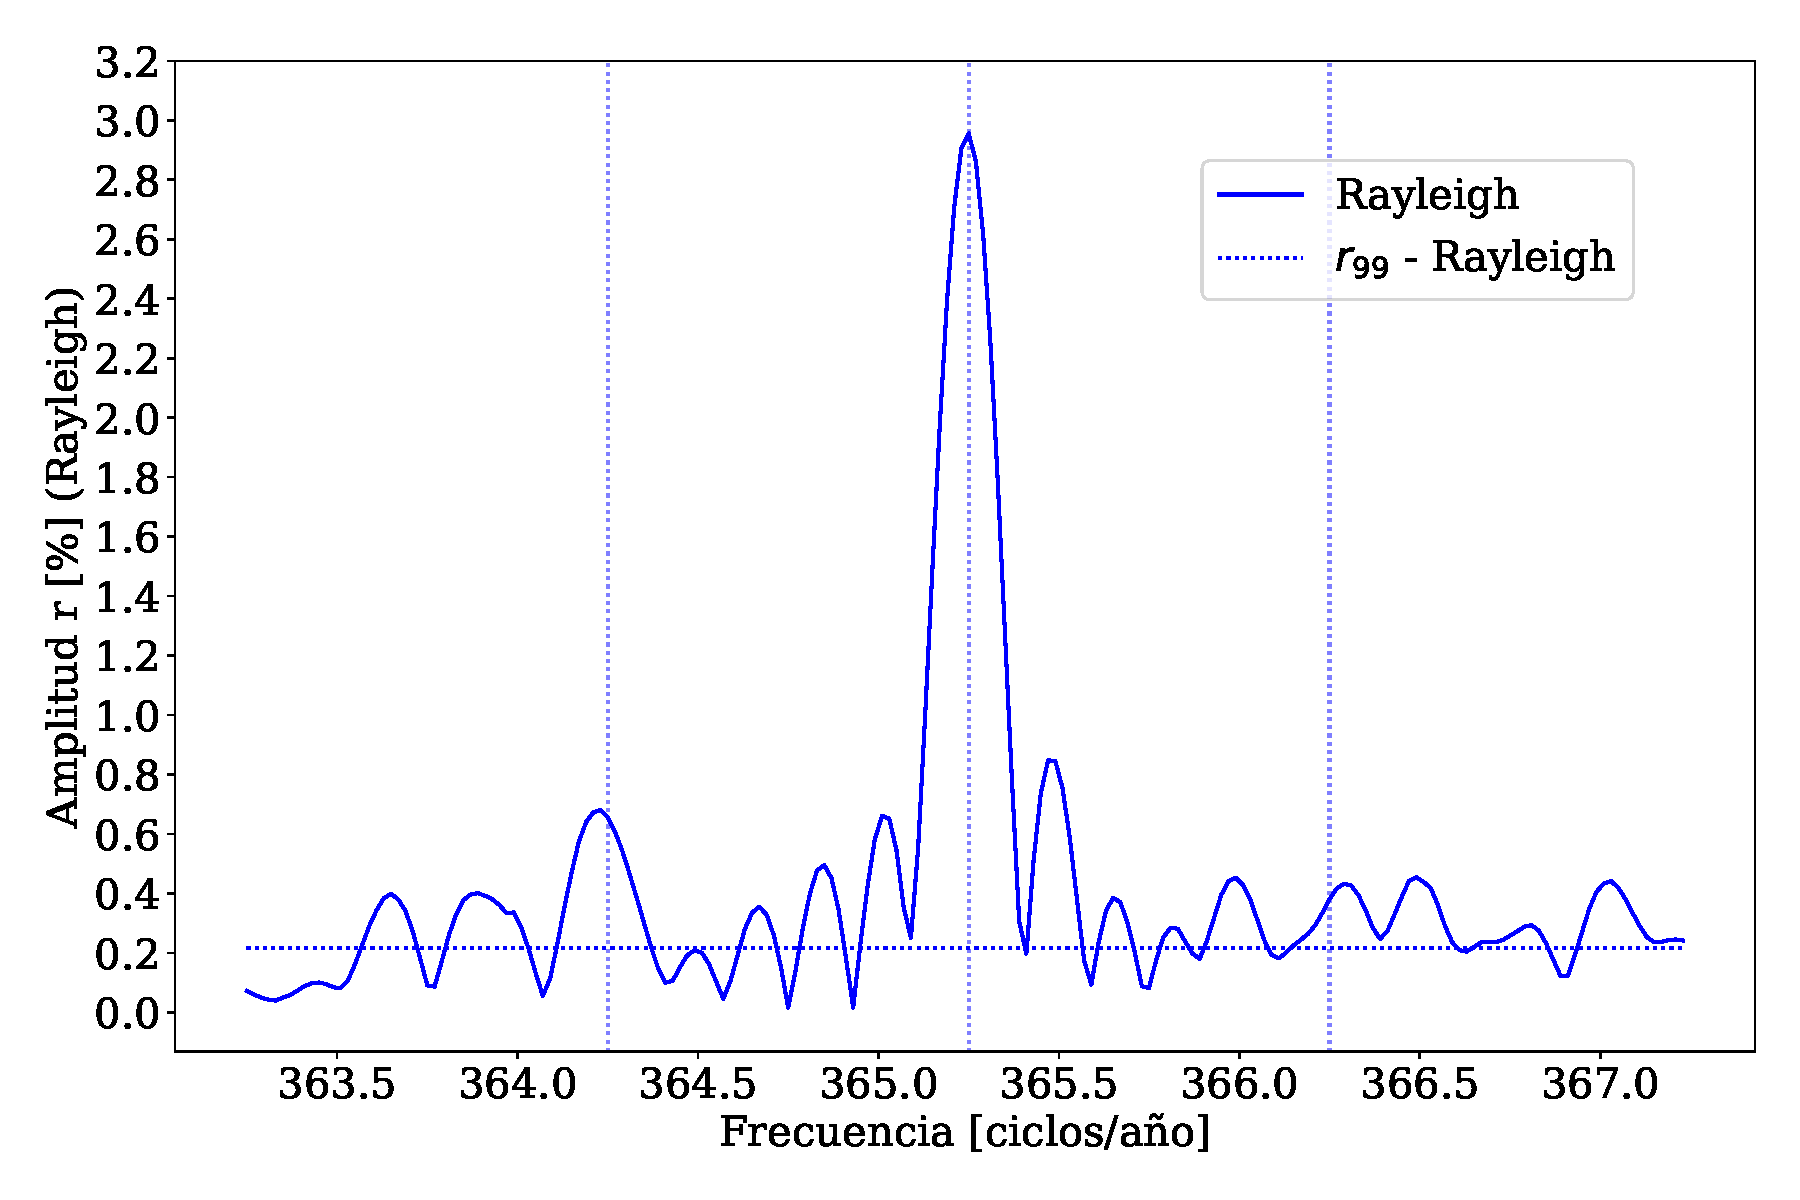
\includegraphics[width=0.4955\textwidth]{plot_bin_1_barrido_v1_Ray.pdf}
        \end{center}
        \caption{Barrido de frecuencias en el rango 0.25 EeV - 0.5 EeV .}
        \label{fig:primer_barrido_EW_Ray}
    \end{small}
\end{figure}    

\begin{figure}[H]
    \begin{small}
        \begin{center}
            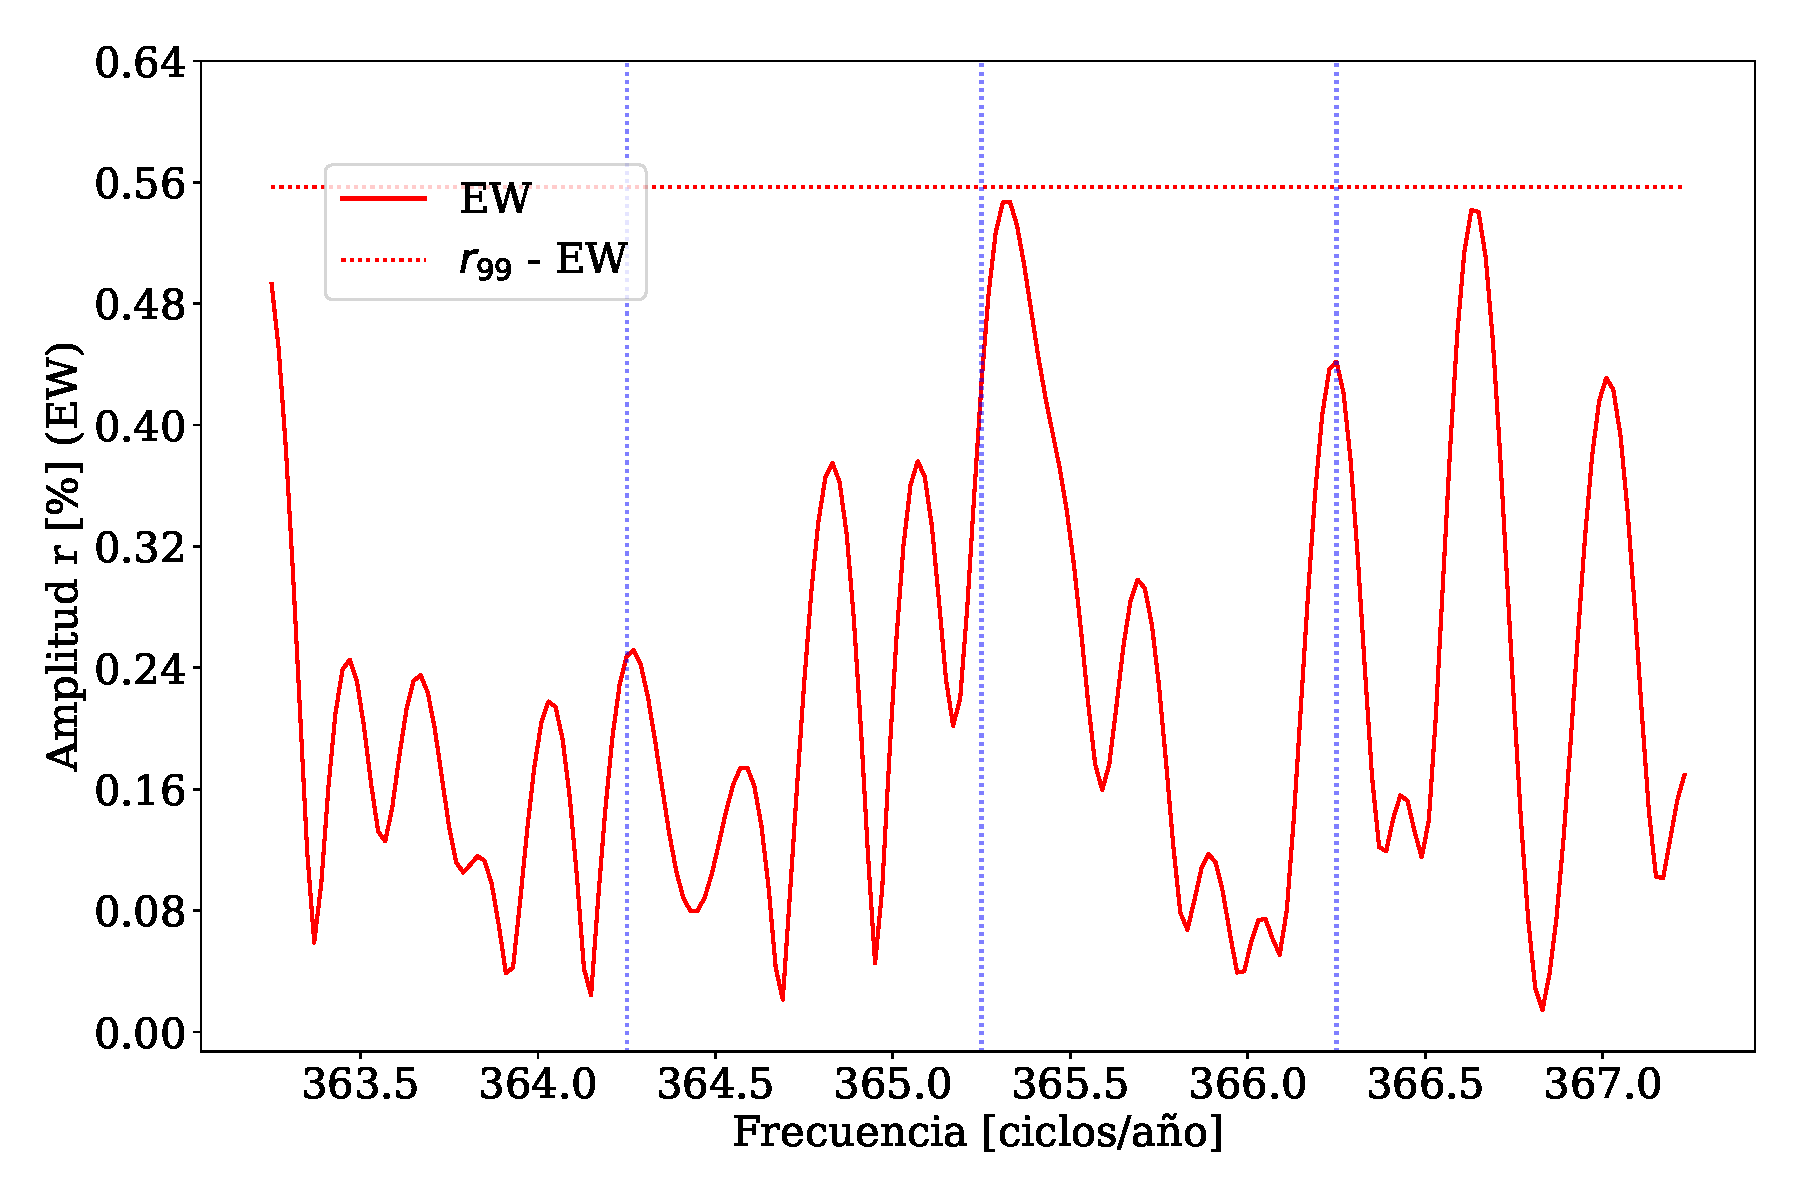
\includegraphics[width=0.4955\textwidth]{plot_bin_2_barrido_v3_EW.pdf}
            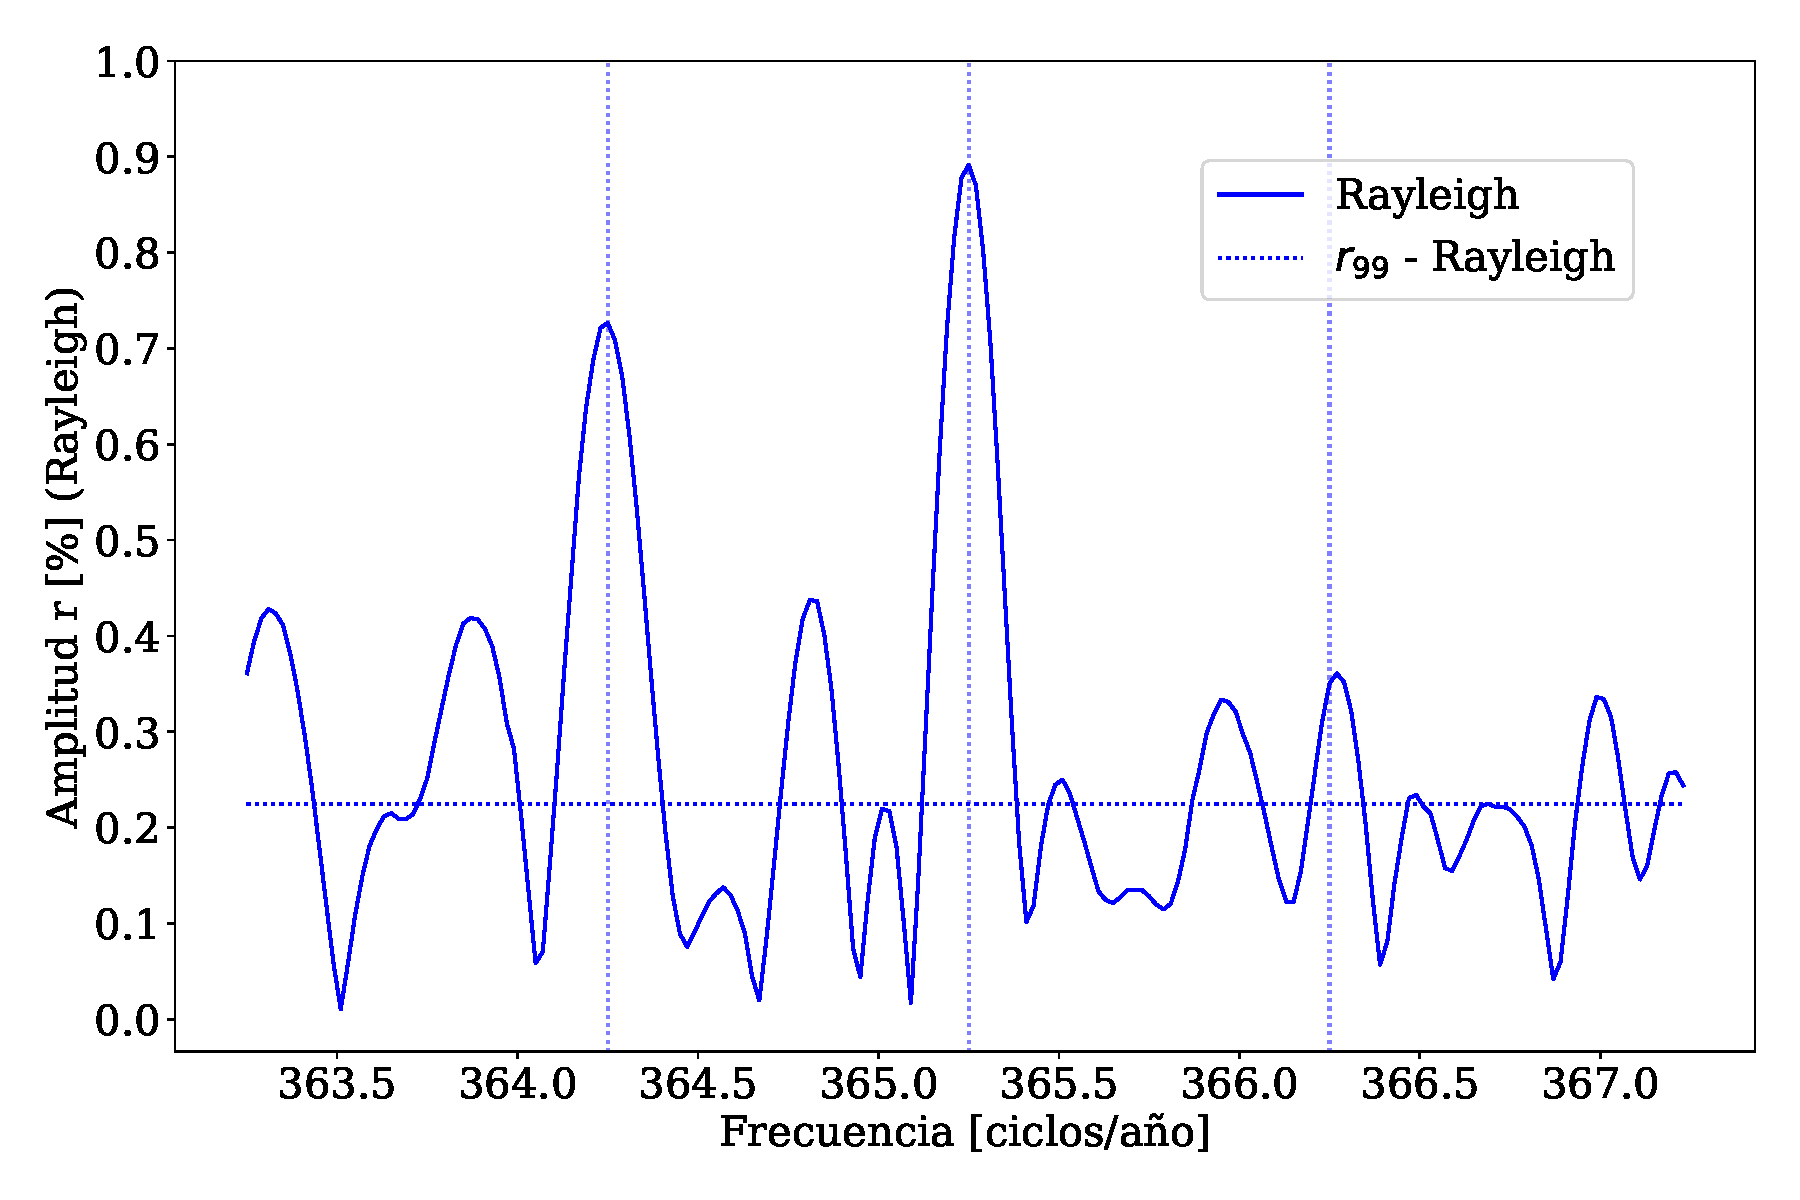
\includegraphics[width=0.4955\textwidth]{plot_bin_2_barrido_v1_Ray.pdf}
        \end{center}
        \caption{Barrido de frecuencias en el rango 0.5 EeV - 1 EeV .}
        \label{fig:segundo_barrido_EW_Ray}
    \end{small}
\end{figure}    

\begin{figure}[H]
    \begin{small}
        \begin{center}
            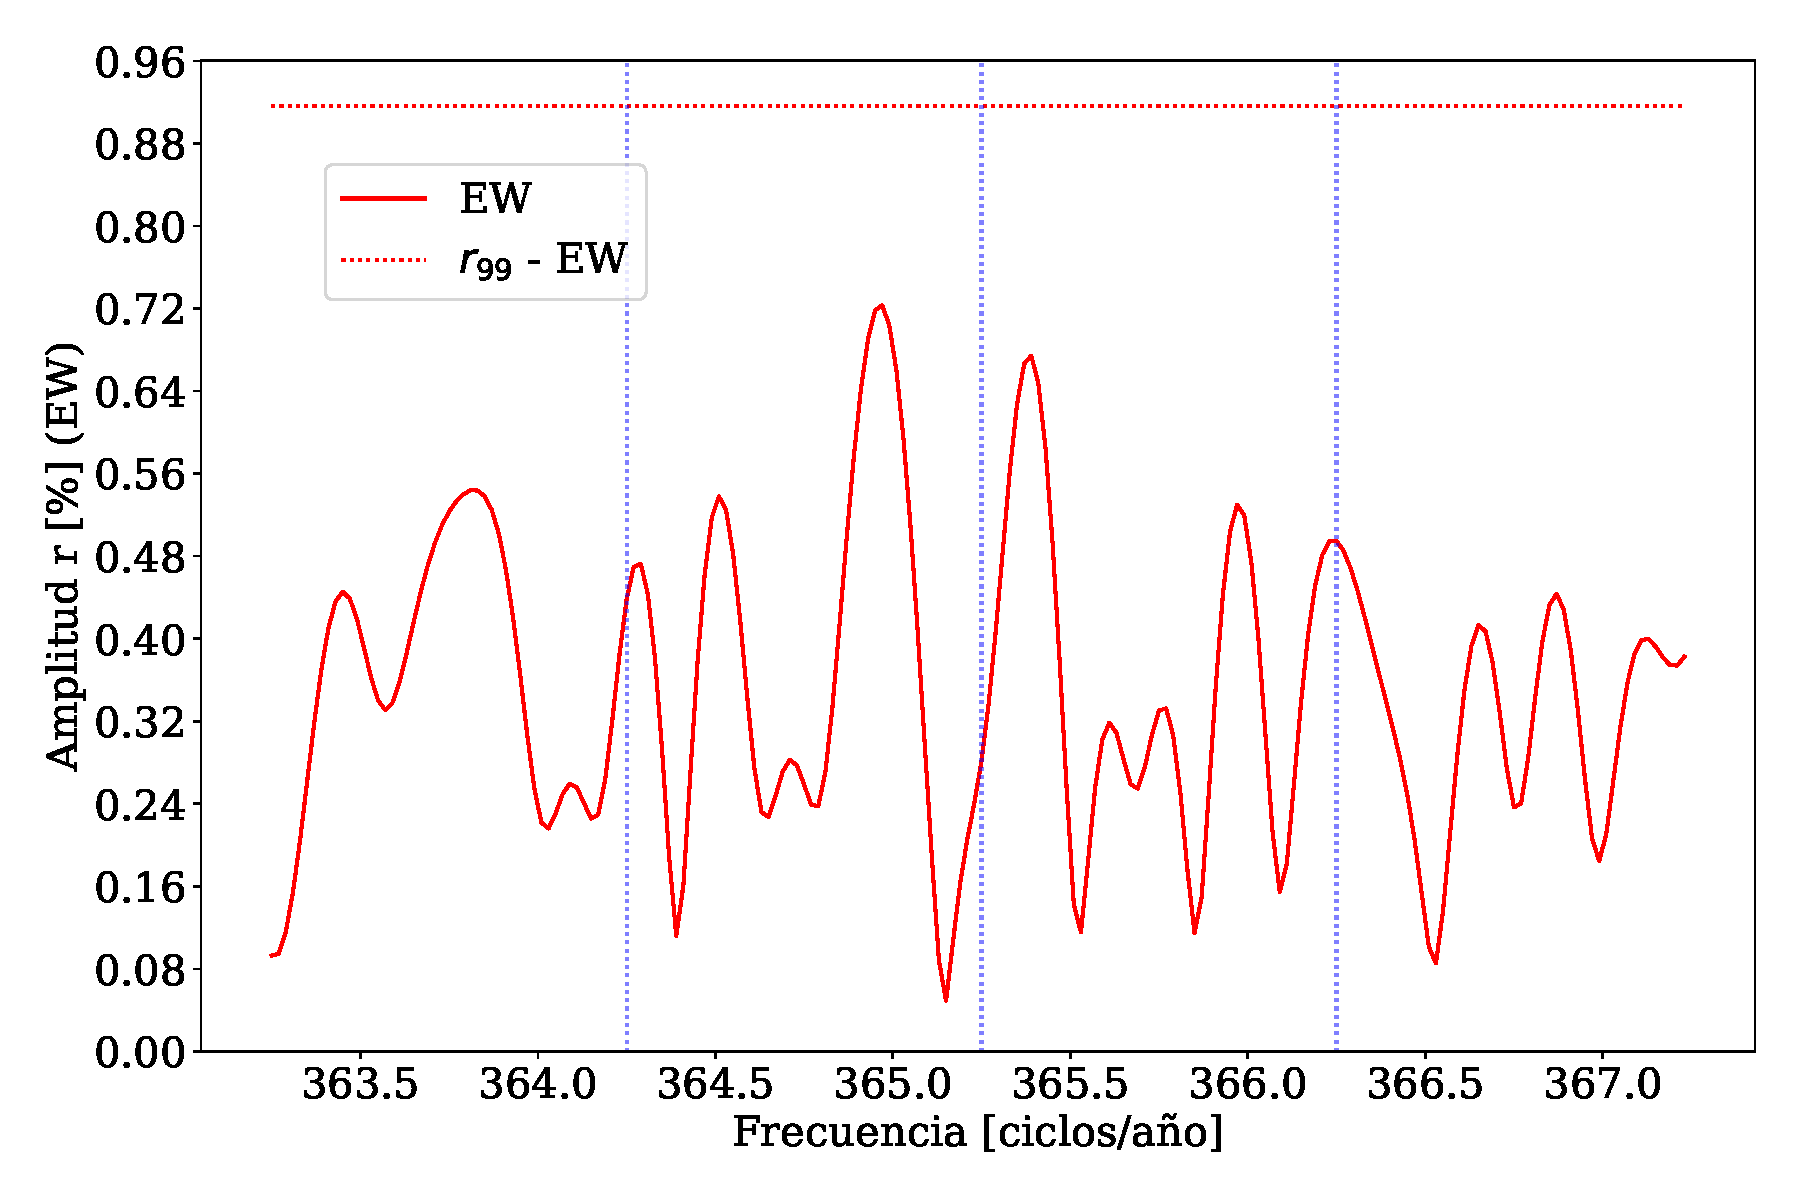
\includegraphics[width=0.4955\textwidth]{plot_bin_3_barrido_v3_EW.pdf}
            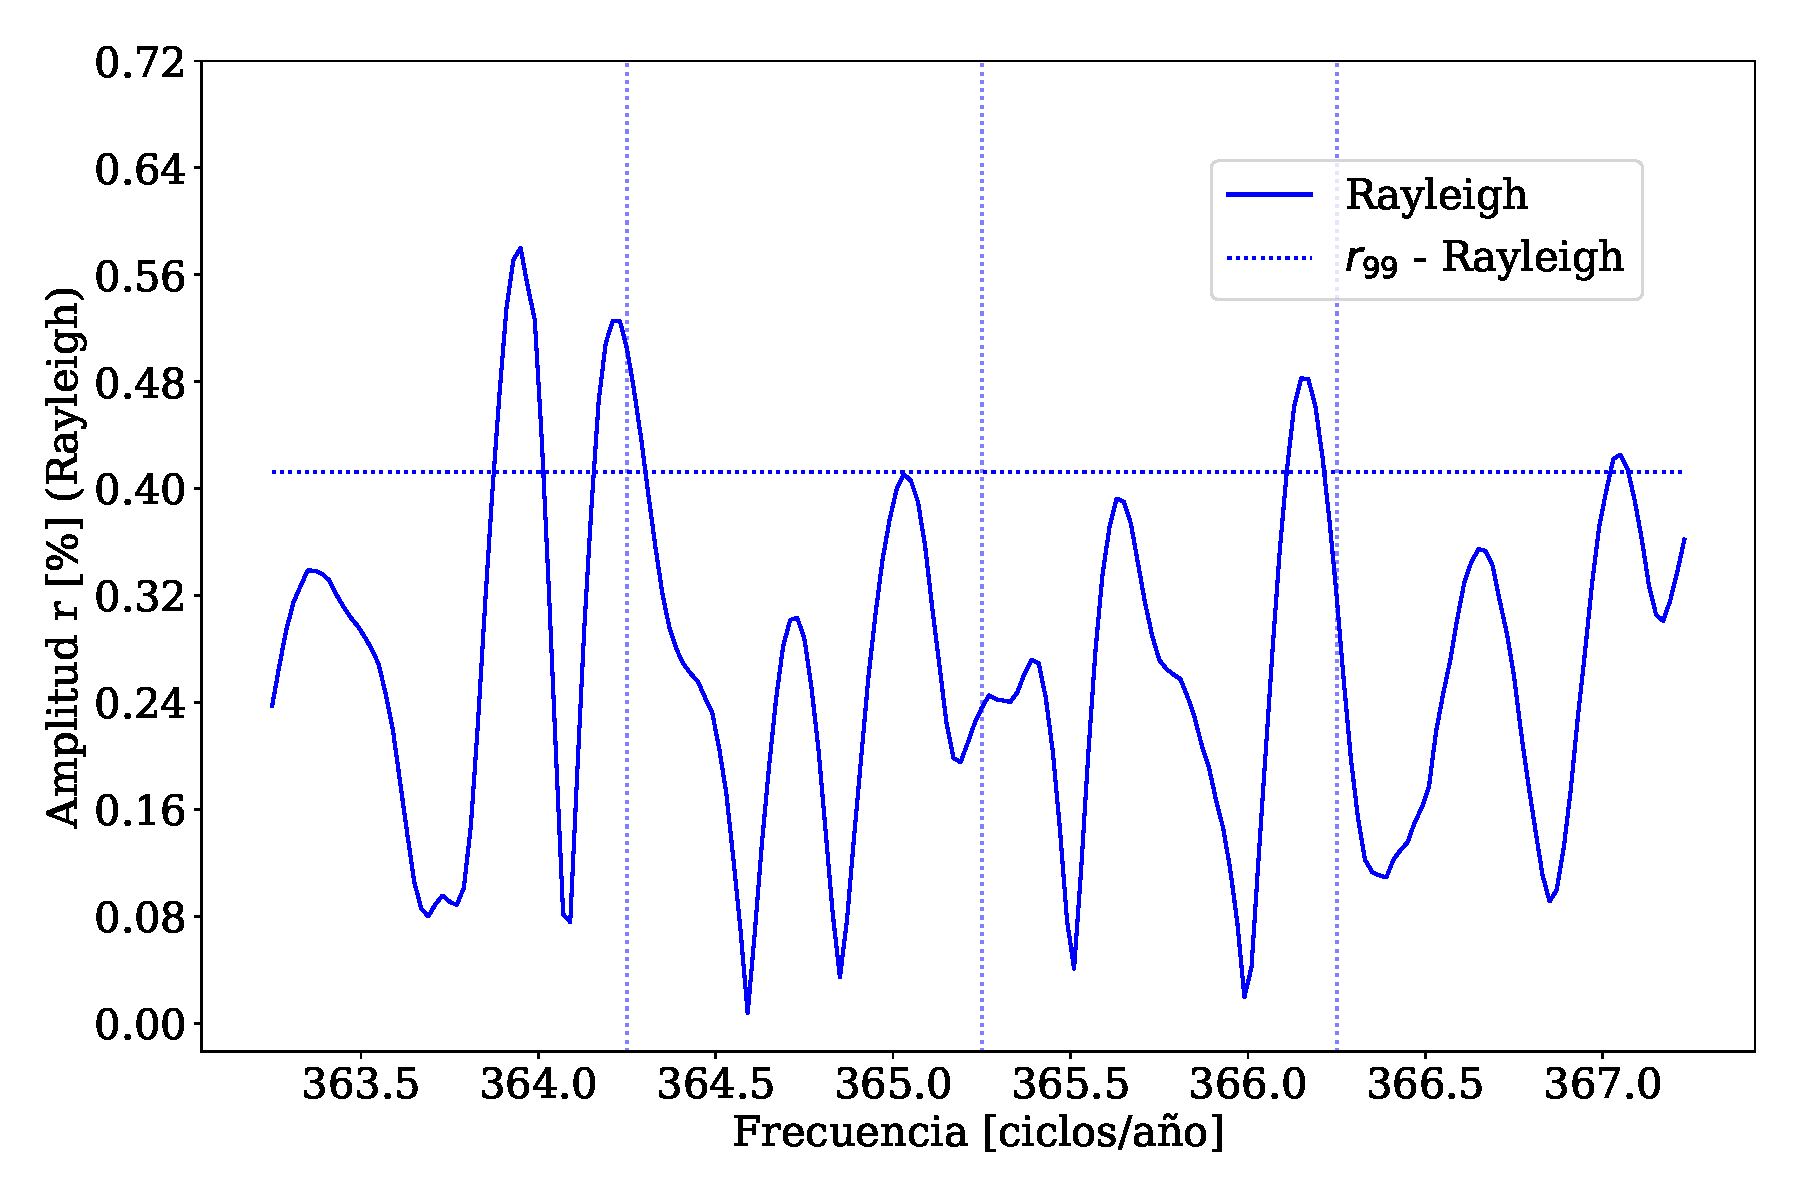
\includegraphics[width=0.4955\textwidth]{plot_bin_3_barrido_v1_Ray.pdf}
        \end{center}
        \caption{Barrido de frecuencias en el rango 1 EeV - 2 EeV .}
        \label{fig:tercer_barrido_EW_Ray}
    \end{small}
\end{figure}    

